\documentclass[12pt]{article}
\usepackage[margin=1.0in]{geometry}
\usepackage[utf8]{inputenc}
\usepackage[T1]{fontenc}
\usepackage{lmodern}
\usepackage[spanish]{babel}
\usepackage{amsmath}
\usepackage{graphicx}
\usepackage{multicol}

\title{\LaTeX\ \textsc{notas}}

\begin{document}
\date{}
\maketitle


\LaTeX. es un programa diseñado con el proposito de crear documentos (libros, artículos, esritos etc.) en un ambiente matemático.
 
\begin{center}
\section*{Primeros pasos con \LaTeX}
\end{center}

Hay tres linéas fundamentales que todo texto en \LaTeX\ debe tener:\\

\begin{center}
\begin{verbatim}
\documentclass[12pt]{article}
\begin{document}

Aca va mi articulo

\end{document}
\end{verbatim}
\end{center}

La primera le dice al programa que clase de documento se va a escribir, en este caso es un art\'iculo.
La segunda indica el inicio del documento mientras que la tercera denota el fin del documento. Entre la segunda 
y la tercera linéa va a ir todo nuestro documento.

\begin{center}
\section*{Margenes:}
\end{center}

Para editar las margenes hay que usar el siguiente paquete:\\

\verb"\usepackage[margin=1.0in]{geometry}"
Donde \verb"margin" es el valor en pulgadas de la margen.


\section*{Idioma:}


Para cambiar de idioma se deben incluir los siguientes paquetes:\\
\verb"\usepackage[utf8]{inputenc}"\\
\verb"\usepackage[T1]{fontenc}"\\
\verb"\usepackage{lmodern}"\\
\verb"\usepackage[spanish]{babel}"\\

\begin{center}
\section*{Tipo de letra y tamaño}
\end{center}


\subsection*{Tipo de letra}


\LaTeX\ 	 trae predeterminadas 7 tipos de letras que son:\\
\verb"\textbf" \textbf{Hola}\\
\verb"\textit" \textit{Hola}\\
\verb"\textsc" \textsc{Hola}\\
\verb"\textsf" \textsf{Hola}\\
\verb"\textsl" \textsl{Hola}\\
\verb"\texttt" \texttt{Hola}\\
\verb"\textrm" \textrm{Hola}\\

\subsection*{Tamaño de letra}

Para cambiar el tamaño de la letra se debe usar la siguiente sintaxis:\\

\begin{verbatim}
\begin{size}
Hola
\end{size}
\end{verbatim}

Donde \verb"size" puede ser:\\

\begin{center}

\begin{tiny}
tiny
\end{tiny} 

\begin{scriptsize}
scriptsize
\end{scriptsize}

\begin{footnotesize}
footnotesize
\end{footnotesize}

\begin{small}
small
\end{small}

\begin{normalsize}
normalsize
\end{normalsize}

\begin{large}
large
\end{large}

\begin{Large}
Large
\end{Large}

\begin{LARGE}
LARGE
\end{LARGE}

\begin{huge}
huge
\end{huge}

\begin{Huge}
Huge
\end{Huge}

\end{center}

\begin{center}
\section*{Secciones}
\end{center}

Para crear secciones dentro de un documento usamos:

\begin{verbatim}
\section{Nombre de la secci\'on}
\end{verbatim}

Por ejemplo esta seccion se llama \textbf{Secciones}.

Tambien podemos crear subsecciones \& subsubsecciones:



\subsection{Soy una subsección}
\begin{verbatim}
\subsection{Nombre de la subsecci\'on}
\end{verbatim}

\subsubsection{Soy una subsubsección}
\begin{verbatim}
\subsubsection{Nombre de la subsubseccion}
\end{verbatim}

\begin{center}
\section*{Ecuaciones y simbolos matem\'aticos}
\end{center}

\subsection*{Simbolos matem\'aticos:}

En general los simbolos matem\'aticos empiezan con un \verb" \" , por ejemplo algunos de los simbolos
mas usados se escribiran:\\

\begin{center}
\begin{tabular}{|c|c|}
\hline
Simbolo & Sintaxis \\\hline
 $\pm$  & \verb"\pm" \\\hline
 $\mp$  & \verb"\mp" \\\hline
$\times$ & \verb"\times" \\\hline
$\div$ & \verb"\div" \\\hline
$\leq$ & \verb"\leq" \\\hline
$\geq$ & \verb"\geq" \\\hline
$\equiv$ & \verb"\equiv" \\\hline
$\simeq$ & \verb"\simeq" \\\hline
$\sum$ & \verb"\sum" \\\hline
$\bigotimes$ & \verb"\bigotimes" \\\hline
$\int$ & \verb"\int" \\\hline
$\oint$ & \verb"\oint" \\\hline
$\partial$ & \verb"\partial" \\\hline
$\hbar$ & \verb"\hslash" \\\hline
$\forall$ & \verb"\forall" \\\hline
$\infty$ & \verb"\infty" \\\hline

\end{tabular}
\end{center}

\subsection*{Ecuaciones:}

Para introducir una ecuaci\'on en el texto primero debemos incluir el siguiente paquete:\\

\verb"\usepackage{amsmath}"

Y luego inicializar la ecuacion así:

\begin{verbatim}
\begin{equation}\label{eq:1.1}
\vec{F} = m \ddot{\vecx}
Esto es una ecuación
\end{equation}
\end{verbatim}

La anterior sintaxis arrojaria el siguiente resultado:

\begin{equation}\label{eq:1.1}
\vec{F} = m \ddot{\vec{x}}
\end{equation}

Donde el label me permite referenciar la ecuaci\'on desde cualquier parte del texto así Eq.\ref{eq:1.1}  

\section*{Figuras}

En muchos textos inclusive no en ciencias las figuras hacen parte escencial para descrbir de manera clara el mensaje
del texto. En \LaTeX  es necesario incluir el paquete \verb"graphicx" para tener las herramientas basicas para hacer graficas:\\

\verb"\usepackage{graphicx}"\\

Ejemplo:\\

\begin{verbatim}
\begin{figure}\label{fig:PhDComics}% Aca defino mi figura y la referencio 
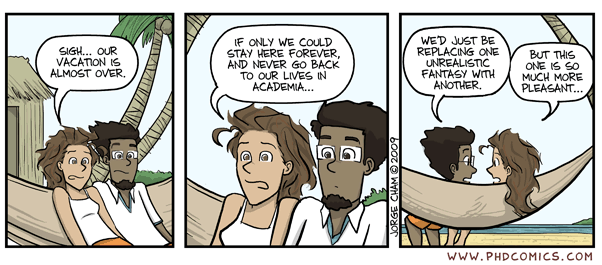
\includegraphics[scale=0.8]{f1.png} % Inserto la imagen y defino su tamaño.
\caption{Your vacations?}% Este es la descripción de mi figura.
\end{figure} % termino de insertar la imagen.
\end{verbatim}

\begin{figure}\label{fig:PhDComics}
\begin{center}
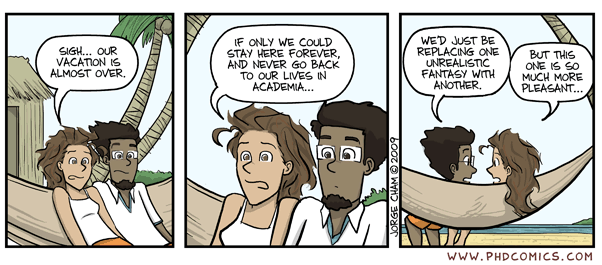
\includegraphics[scale=0.8]{f1.png}
\caption{Your vacations?}
\end{center}
\end{figure}

Para referenciar la figura dentro del texto uso \verb+\ref{fig:PhDComics}+ esto quedar\'a as\'i:\\
En la Fig.\ref{fig:PhDComics} vemos unas lindas vacaciones$!$

\section*{Tablas}

Al igual que las figuras varias las tablas son utilies para presentar informaci\'on de una mejor manera, en muchos 
casos resumiendo caracteristicas.\\

Ejemplo:\\

\begin{verbatim}
\begin{table}\label{tab:distance}
\begin{center}
\begin{tabular}{|c|c|}% cada c define una columna, en este ejemplo hay dos columnas.
\hline
Tiempo ($s$) & Distancia $m$ \\
\hline
1 & 20\\
\hline
3 & 50\\
\hline
\vdots & \vdots \\
\end{tabular}
\caption{Tiempo y distancias}
\end{center}
\end{table}

\end{verbatim}

\begin{table}\label{tab:distance}
\begin{center}
\begin{tabular}{|c|c|}
\hline
Tiempo ($s$) & Distancia $m$ \\
\hline
1 & 20\\
\hline
3 & 50\\
\hline
\vdots & \vdots \\
\end{tabular}
\caption{Tiempo y distancias}
\end{center}
\end{table}

Table \ref{tab:distance} muestra..

\section*{Columnas}

Agregar \verb"\usepackage{multicol}"

\begin{multicols}{2}
"Murakami was born in Japan during the post–World War II baby boom. Although born in Kyoto, he spent his youth in Shukugawa (Nishinomiya), Ashiya and Kobe. His father was the son of a Buddhist priest, and his mother the daughter of an Osaka merchant. Both taught Japanese literature.

Since childhood, Murakami has been heavily influenced by Western culture, particularly Western music and literature. He grew up reading a wide range of works by American writers, such as Kurt Vonnegut, Richard Brautigan and Jack Kerouac. These Western influences distinguish Murakami from other Japanese writers.

Murakami studied drama at Waseda University in Tokyo, where he met his wife, Yoko. His first job was at a record store, much like Toru Watanabe, the narrator of Norwegian Wood. Shortly before finishing his studies, Murakami opened a coffeehouse and jazz bar, the Peter Cat, in Kokubunji, Tokyo, which he ran with his wife from 1974 to 1981—again, not unlike the protagonist in his later novel South of the Border, West of the Sun.

Many of his novels have themes and titles that invoke classical music, such as the three books making up The Wind-Up Bird Chronicle: The Thieving Magpie (after Rossini's opera), Bird as Prophet (after a piano piece by Robert Schumann usually known in English as The Prophet Bird), and The Bird-Catcher (a character in Mozart's opera The Magic Flute). Some of his novels take their titles from songs: Dance, Dance, Dance (after The Dells' song, although it is widely thought it was titled after the Beach Boys tune), Norwegian Wood (after The Beatles' song) and South of the Border, West of the Sun (after the song "South of the Border").

Murakami is a marathon runner and triathlon enthusiast, though he did not start running until he was 33 years old. On June 23, 1996, he completed his first ultramarathon, a 100-kilometer race around Lake Saroma in Hokkaido, Japan. He discusses his relationship with running in his 2008 memoir What I Talk About When I Talk About Running" \cite{Wiki}
\end{multicols}


\section*{Bibliograf\'ia}

La Bibliografia se puede hacer de dos maneras, corta para trabajos e informes, o larga para articulos y libros.\\

Esta es al forma corta:\\
Se referencia así \cite{Latex} \verb"\cite{Taylor}".




Para libros y art\'iculos:\\

Se crea un archivo .bib donde esta toda la bibliograf\'ia en este formato:

\begin{verbatim}
@BOOK{book,
	    AUTHOR = "author",
	    TITLE = "book title",
	    PUBLISHER = {publishing company},
	    ADDRESS = {where published},
	    YEAR = year published}

\end{verbatim}

Y se referencia as\'i:\\
\cite{book}
\verb"\cite{book}"

Para compilar usamos:\\

\begin{verbatim}
    pdflatex latex_source_code.tex
    bibtex latex_source_code.aux
    pdflatex latex_source_code.tex
    pdflatex latex_source_code.tex
\end{verbatim}

Ver mas en: \cite{wiki}

%\begin{center}
\section*{Tips:}
%-\end{center}

\begin{itemize}
\item Para dejar un espacio distanciado entre lineas se debe usar \verb"\\" al final de cada linea.
\item Para escribir simbolos o ecuaciones matemáticas en el texto se debe usar el simbolo \$ \verb"$\dfrac{dx}{dt}$"   $\dfrac{dx}{dt}$
\item Para comentar lineas se utiliza el simbolo de porcentaje \%.
\end{itemize}

\bibliography{references}



\begin{thebibliography}{5}
\bibliographystyle{plainnat}
\bibitem{Tutorial}http://www.latex-tutorial.com/\\
\bibitem[LatexOficial]{Latex}http://www.latex-project.org/\\
\bibitem{Templates}http://www.latextemplates.com/\\
\bibitem{Wiki}https://en.wikipedia.org/wiki/Haruki\verb"_"Murakami
\bibitem{wiki}\verb"https://en.wikibooks.org/wiki/LaTeX/Bibliography_Management"
\end{thebibliography}

\end{document}
